%%%%%%%%%%%%%%%%%%%%%%%%%%%%%%%%%%%%%%%%%%%%%%%%%%%%%%
%\section{Human Activity Recognition}
%%%%%%%%%%%%%%%%%%%%%%%%%%%%%%%%%%%%%%%%%%%%%%%%%%%%%%

\subsection{Method}

Explain general approaches to human activity recognition.

\begin{figure}[htbp]
\centering
\subfigure[Classification Overview]{
\label{fig:integrated_har_overview}
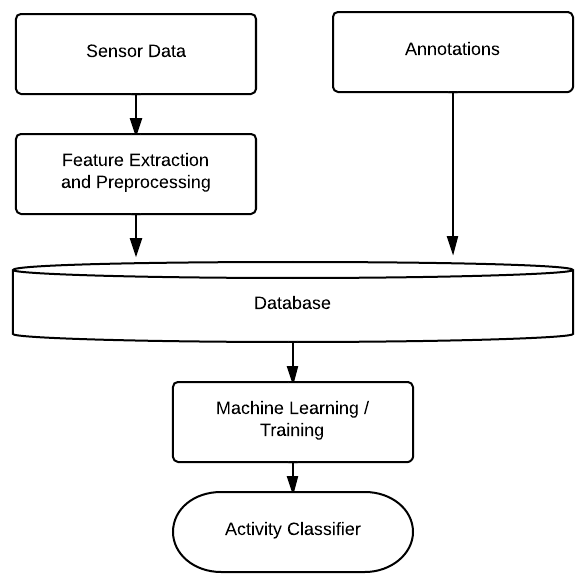
\includegraphics[width=0.5 \textwidth]{img/har/classification_overview.png}
}
\subfigure[Integrated HAR Classifier]{
\label{fig:integrated_har_overview}
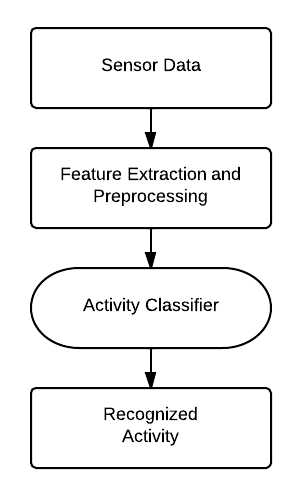
\includegraphics[width=0.25 \textwidth]{img/har/integration_overview.png}
}
\caption{Overview Human Activity Recognition}
\end{figure}

\subsection{Related Work}
Evaluation methods and resulted quality in the literature.

\subsection{Component Description}

Architecture Description.

\begin{figure}[htbp]
\centering
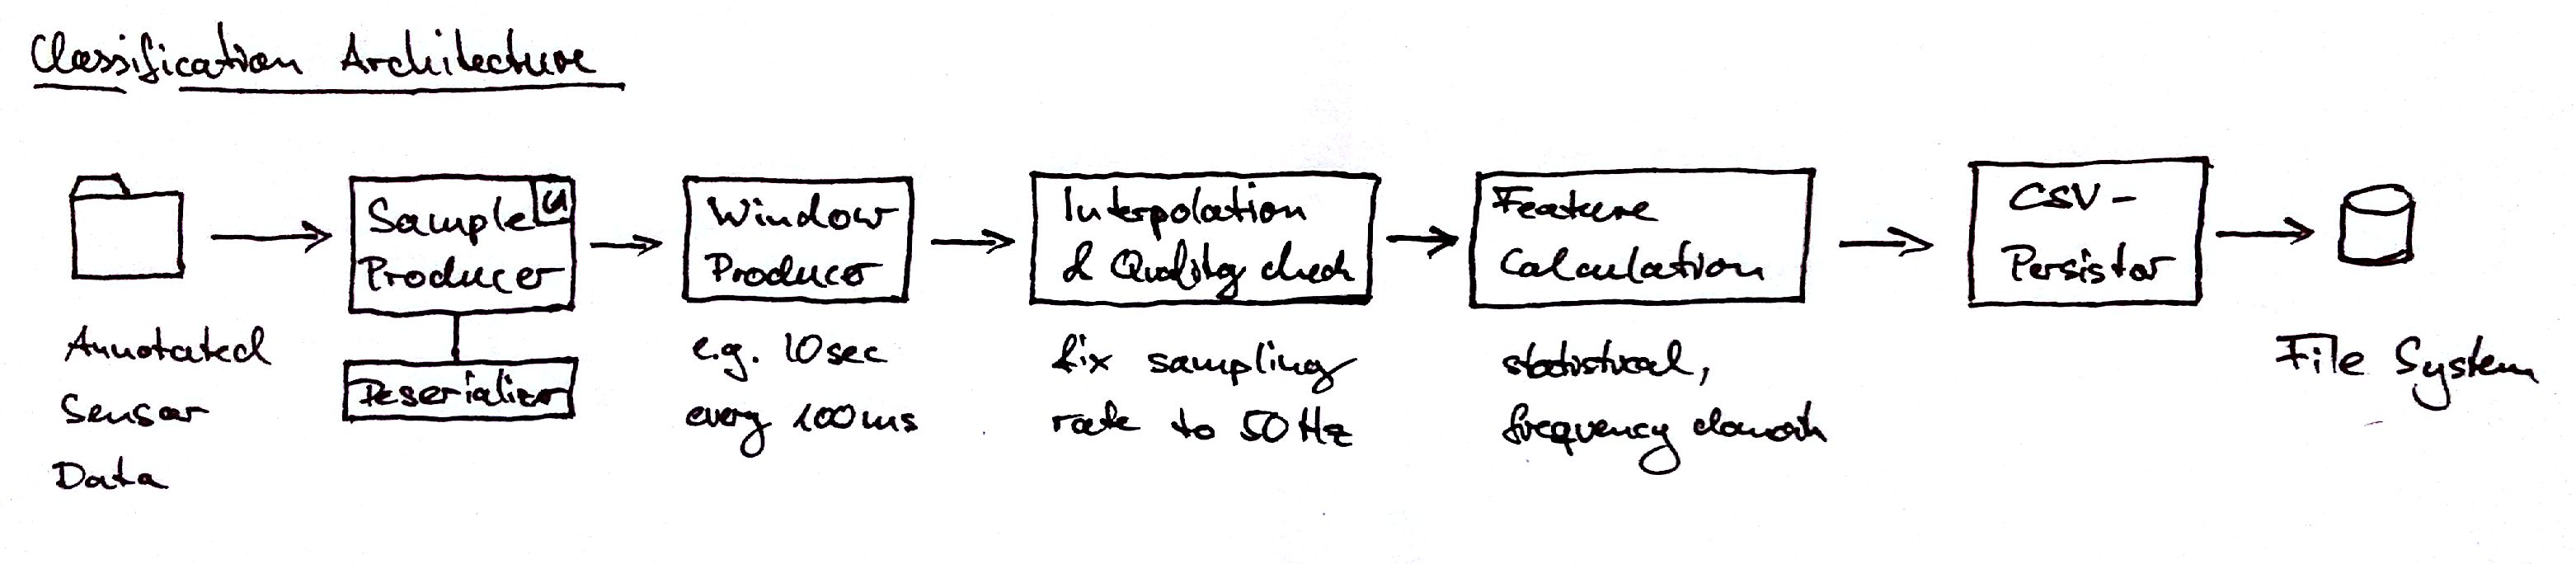
\includegraphics[width=\textwidth]{img/har/classification_architecture.jpg}
\caption{Classification Architecture}\label{fig:classification_architecture}
\end{figure}

\begin{figure}[htbp]
\centering
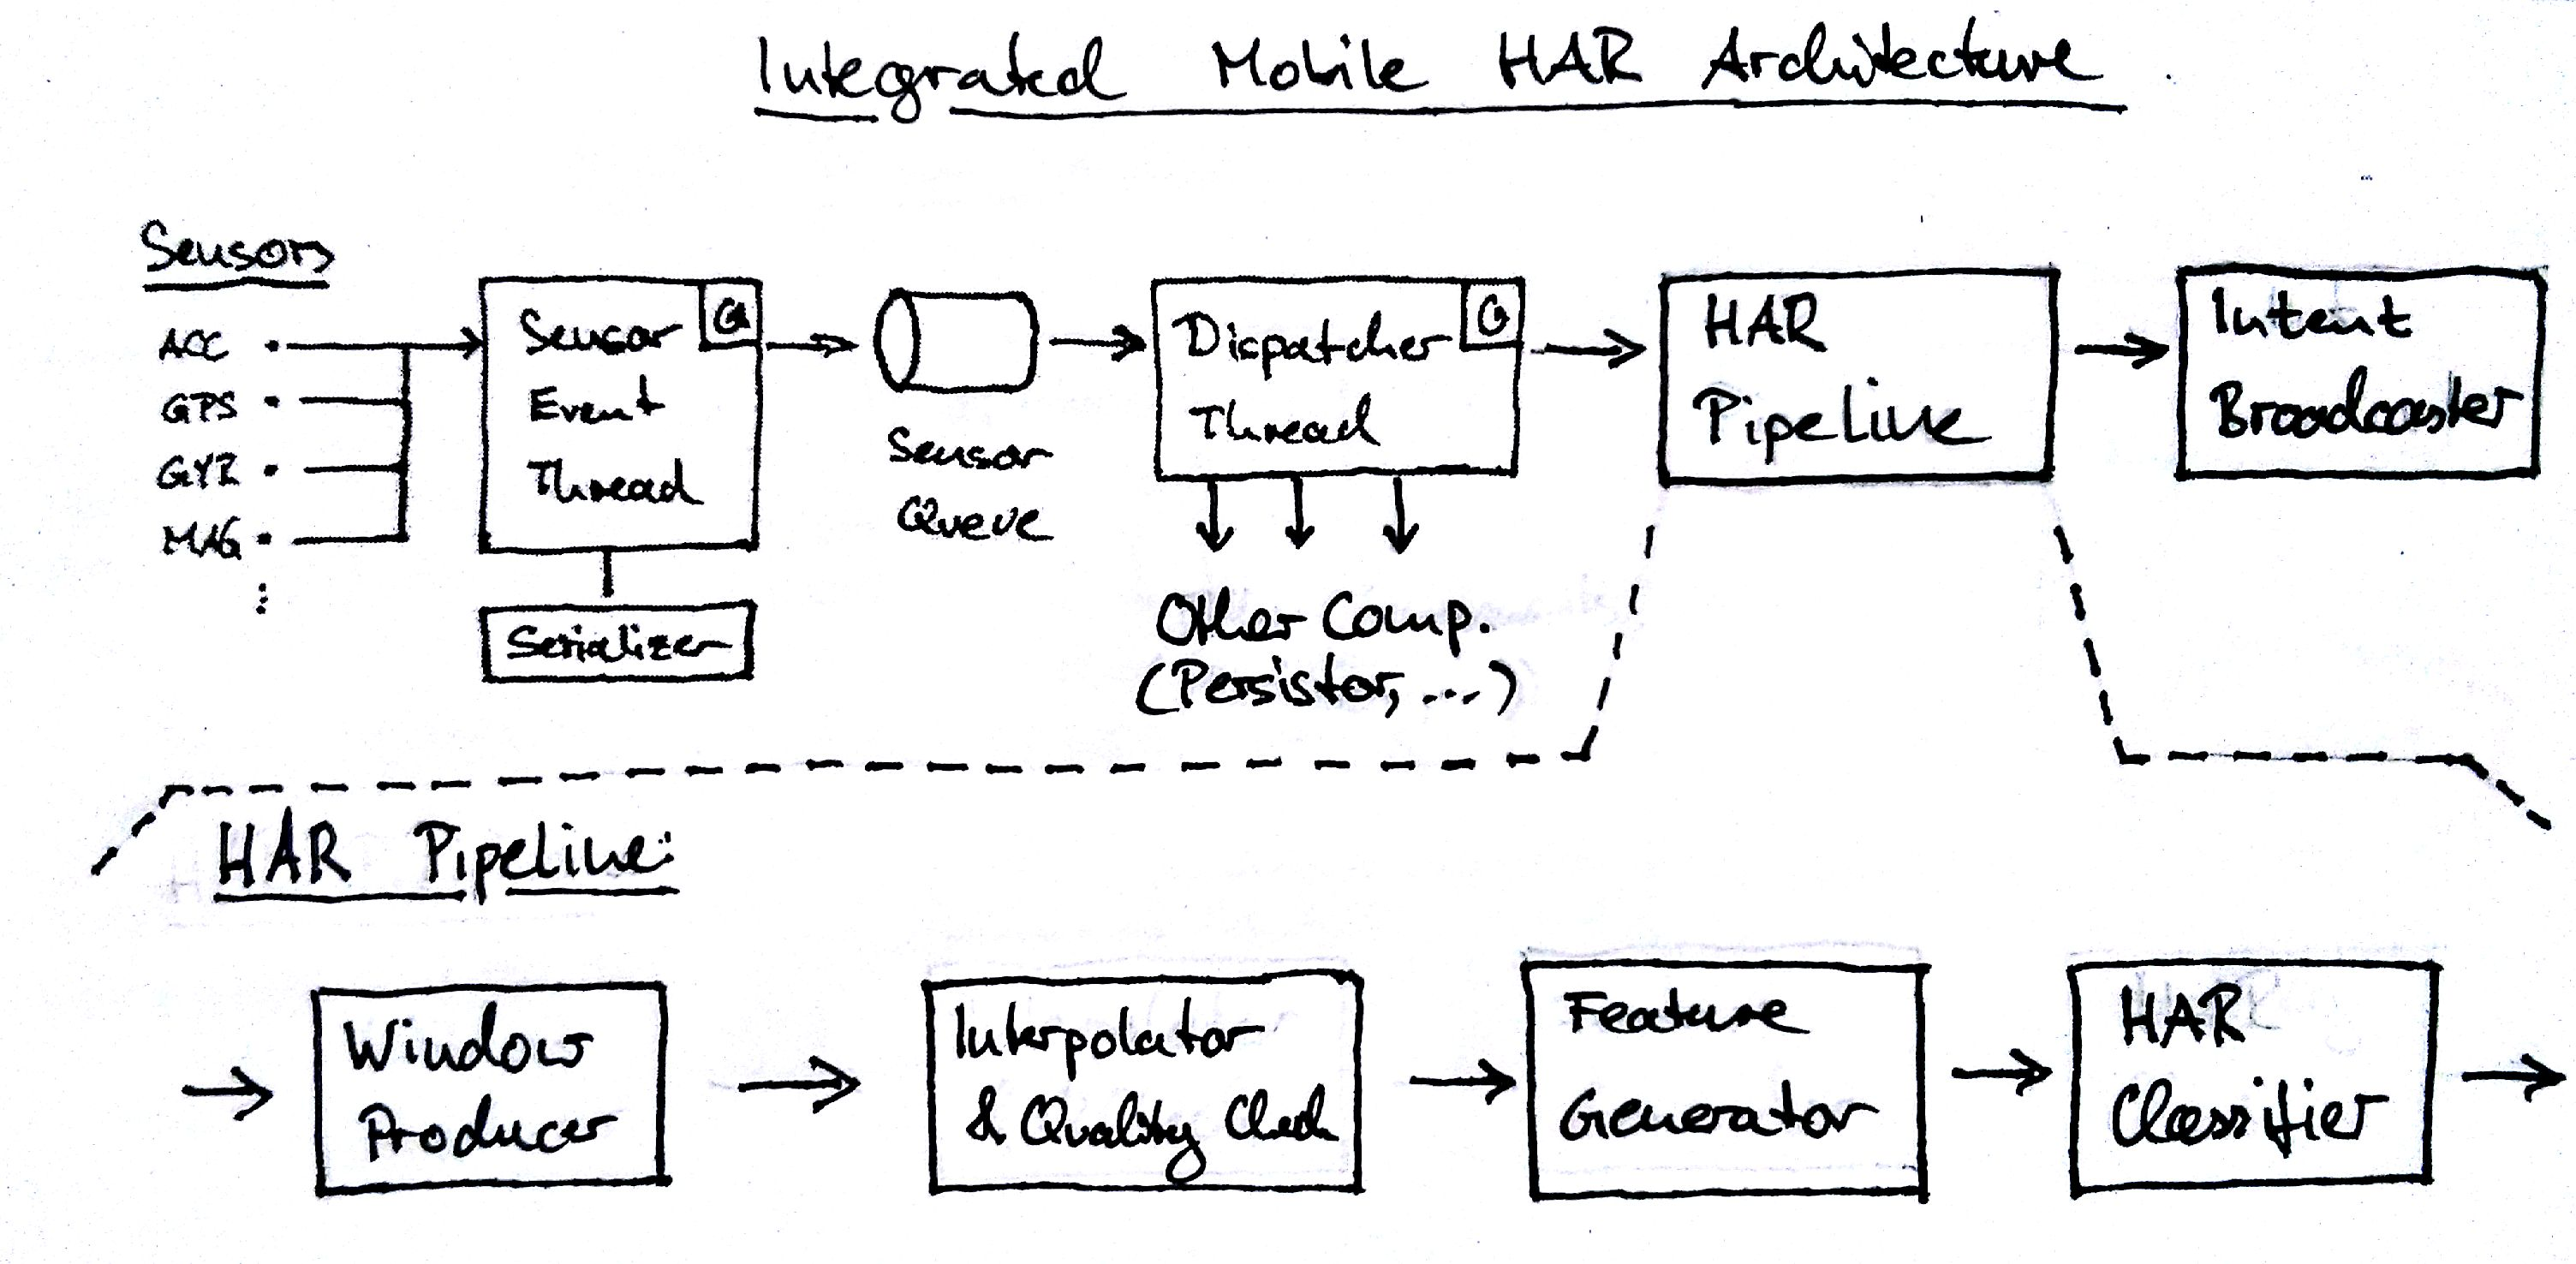
\includegraphics[width=\textwidth]{img/har/integration.jpg}
\caption{Integrated HAR Architecture}\label{fig:integrated_har}
\end{figure}

% TODO CE
% Describe the component implementation.
% This can be done in a similar fashion like the sensor collector
% further up: Add Bullet point list for the individual components.
% And describe them in one or two sentences.
% * Add a list for the features we use in the current implementation
% * Describe how we train the decision tree classifier using WEKA.
%   Add a screenshot of the results. 
% * Describe how we integrate the classifier into the application


\subsection{Evaluation}

Comparison of our classifier with literature on the basis of external
data sets.


%%% Local Variables:
%%% mode: latex
%%% TeX-master: "../D1-2"
%%% End:
